% Chapter 2

\chapter{Reconocimiento de iris} % Main chapter title

\label{Capítulo 2} % For referencing the chapter elsewhere, use \ref{Chapter2} 

%----------------------------------------------------------------------------------------

% Define some commands to keep the formatting separated from the content 
%\newcommand{\keyword}[2]{\textbf{#2}}
%\newcommand{\tabhead}[2]{\textbf{#2}}
%\newcommand{\code}[2]{\texttt{#2}}
%\newcommand{\file}[2]{\texttt{\bfseries#2}}
%\newcommand{\option}[2]{\texttt{\itshape#2}}

%----------------------------------------------------------------------------------------

La creciente demanda en cuanto a sistemas de seguridad se refiere unido a la necesidad de satisfacer las exigencias que estos presentan ha permitido que la identificación de personas basada en características biométricas haya experimentado un creciente desarrollo durante las últimas décadas. Los sistemas biométricos tienen el objetivo de realizar una correcta identificación de cada individuo, utilizando para ello diferentes características fisiológicas o de comportamiento del mismo tales como huellas digitales, rostro, patrón de escritura, retina, iris, geometría de la mano, etc. \\

Debido a las propiedades de única, invariable y accesible que presenta las características del patrón del iris, la identificación personal basada en este modelo estructural se ha convertido en una de las técnicas mas confiable y segura dentro del paradigma del reconocimiento de personas\cite{Reference1} \cite{Reference2} \cite{Reference3} \cite{Reference4} \cite{Reference5}. \\

Actualmente son muchos los sistemas de reconocimiento basados en el iris desarrollados tanto de manera comercial como no comercial, siendo el distribuido por Iridian Technologies \cite{Reference6} el más existoso comercialmente. Este sistema se basa en los algoritmos patentados y desarrollados por Daugman \cite{Reference1}, los cuales son la base teórica de la mayoría de sistemas de reconocimiento de esta modalidad, y que incluye el desarrollo de todas las etapas que conforman este tipo de sistemas. Existe también una serie de implementaciones de sistemas de reconocimiento de iris no comerciales que aunque no son tan conocidos como el anteriormente comentado es interesante mencionarlos ya que proponen diferentes algoritmos de segmentación, codificación y comparación que algunas librerías los desarrollan. Entre estos podemos destacar los sistemas propuestos por Wildes \cite{Reference4} , Boles y Boashash \cite{Reference2}, Sanchez et al. \cite{Reference7} y Ma et al. \cite{Reference3}.  \\ 


%----------------------------------------------------------------------------------------

\section{Sistemas de reconocimiento}

El amplio campo que abarcan los sistemas de reconocimiento ha generado que se haya ido pasando de los más rudimentarios como el uso de una palabara clave o algún tipo señal, hasta los mas avanzados que actualmente se desempeñan en el área de la biometría. El acto de limitar el acceso a ciertos lugares para unos indivuos concretos o transmitir información de manera segura a la persona indicada, son algunas de las situaciones donde los sistemas de reconocimiento son empleados. Globalmente, su uso viene determinado por dos procesos, un primer proceso de verificación y un segundo proceso de identificación. \\

A través del proceso de verificación se valida la identidad de un individuo comparando si los datos de entrada cumplen con la estructura de tipo de dato que el sistema está esperando. En general, el usuario indicará su identidad mediante un número de identificación personal, un nombre de usuario, un código, un escaner de retina, etc, dependiendo del tipo de sistema de reconocimiento que esté implantado. Posteriormente el sistema realizará una comparación para determinar si el individuo es quien dice ser. Este proceso puede dar lugar a la aparición de dos posibles errores; un falso rechazo (FRR) producido cuando el sistema indica que la información de entrada adquirida del usuario no coindice con la estructura de información que tiene que recibir, cuando realmente si corresponde, y una falsa aceptación (FAR) que es complementario al falso rechazo y es producida cuando el sistema indica que la información de entrada adquirida del usuario si se corresponde con la estructura de información que tiene que recibir, cuando realmente no concuerdan.  \\

Mediante el proceso de identificación, el sistema comprueba que la información de entrada facilitada por el usuario coincide con alguno de los modelos de datos almacenados en la base de datos del mismo. El sistema decidirá si el usuario está o no en la base de datos. Hay que tener en cuenta que este proceso es mucho más costoso computacionalmente que el anterior debido a que será proporcional al número de entradas que contenga la base de datos. \\

Los primeros sistemas de reconocimiento se basaban en simples acciones realizadas por la persona que se quería identificar como una señal con la mano, una señal de luz, un código escrito, una palabra clave, etc, lo que permitía a la otra parte comprobar que la persona era quien dice ser. Pronto comenzaron a surgir los problemas con este tipo de sistemas de reconocimiento ya que eran muy poco seguros y fiables de cara a la persona que obstentaba las credenciales. En esta tesitura, cualquier persona interesada en suplantar la identidad de otra podría reproducir el tipo de señal con la mano o de luz que esta utilizara para acceder con su identidad, del mismo modo que era posible conocer el código empleado así como la palabra clave. También se podría dar el caso de que la persona olvidara el tipo de señal, la palabra o el código que la identifican, impidiendole de esta manera el poder realizar cualquier acción que necesitará de una previa identificación. \\

\begin{figure}[htbp]
\centering
\subfigure[Señal con la mano]{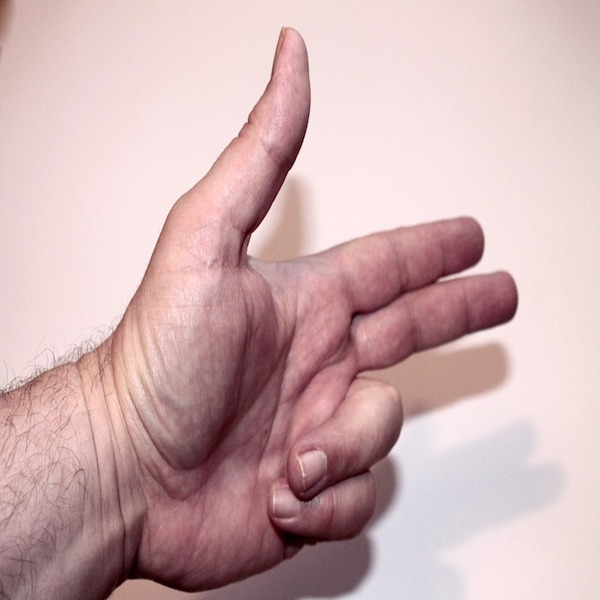
\includegraphics[width=40mm]{tfm-img1}}
\subfigure[Señal con luz]{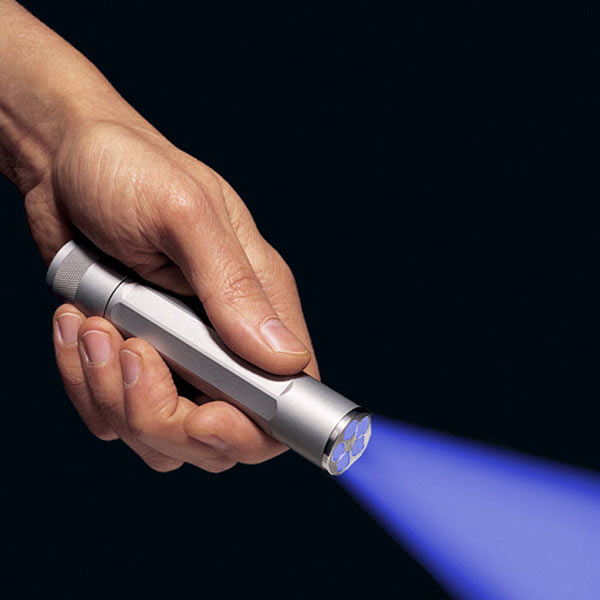
\includegraphics[width=40mm]{tfm-img2}}
\subfigure[Código escrito]{
\includegraphics[width=80mm]{tfm-img3}}
\caption{Primeros sistemas de reconocimiento.} \label{fig:señales}
\end{figure}

Todos estos problemas fueron solventados con la aparición de la tecnología magnética. El que la información estuviese contenida en una banda magnética organizada en diferentes pistas hacía que no se pudiesen dar los casos sucedidos con los sistemas de reconocimientos tradicionales. En este ámbito, el uso de la tarjeta magnética era el medio utilizado en los sistemas de reconocimiento. Una tarjeta que poseía una banda magnética donde se almacenaba un código y que era leído a través de un lector con el que se podía extraer dicha información e identificar rápidamente a la persona que la portaba. Durante muchos años los sistemas de reconocimiento utilizaron este dispositivo como medio donde la información de identificación iba contenida. \\

\begin{figure}[htbp]
\centering
\subfigure[Tarjeta con banda magnética]{
\includegraphics[width=50mm]{tfm-img4}}
\subfigure[Lector de tarjetas por banda magnética]{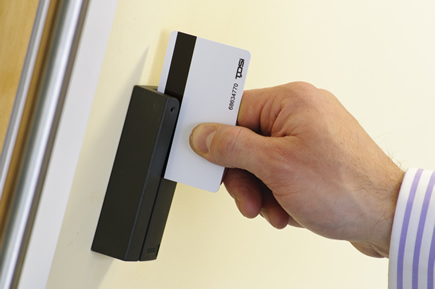
\includegraphics[width=50mm]{tfm-img5}}
\caption{La tecnología magnética en los sistemas de reconocimiento.} \label{fig:señales}
\end{figure}


El gran avance que experimentó la informática y la electrónica con el paso de los años hizo que los sistemas de reconocimiento a través de bandas magnéticas comenzasen a sufrir problemas de seguridad a raiz de la alta posibilidad que existía para suplantarlos. A este problema se unía el desgaste físico que se originaba en las bandas magnéticas a casua de su frecuente uso. Esto podía producir daño en la información almacenada en dichas bandas produciendo errores en la identificación. Fue en este punto cuando la tecnología digital apareció para dar solución a todos los inconvenientes que el uso de la tecnología magnética presentaba. La implantación de los chips digitales en los medios empleados por los sistemas de reconocimiento consiguieron dotar de una mayor seguridad y consistencia a estos sistemas, a la vez que hacía mas rápido todo el proceso de indentificación. Dispositivos como las tarjetas con banda magnética comenzaron incorporar este tipo de tecnología, al igual que los lectores tuvieron que actualizarse para extraer esa información. En este mismo entorno la tecnología digital progresó hasta la conexión entre dispositivos de manera inhalámbrica, es decir, los mismos dispositivos como las tarjetas se comunicaban con los lectores sin contacto físico, solo situándose a corto alcance. \\

\begin{figure}[htbp]
\centering
\subfigure[Tarjeta chip digital]{
\includegraphics[width=40mm]{tfm-img6}}
\subfigure[Lector de tarjetas por chip digital]{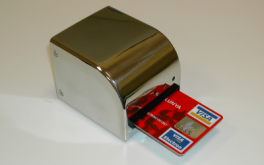
\includegraphics[width=36.3mm]{tfm-img7}}
\subfigure[Lector de tarjetas por chip digital wireless]{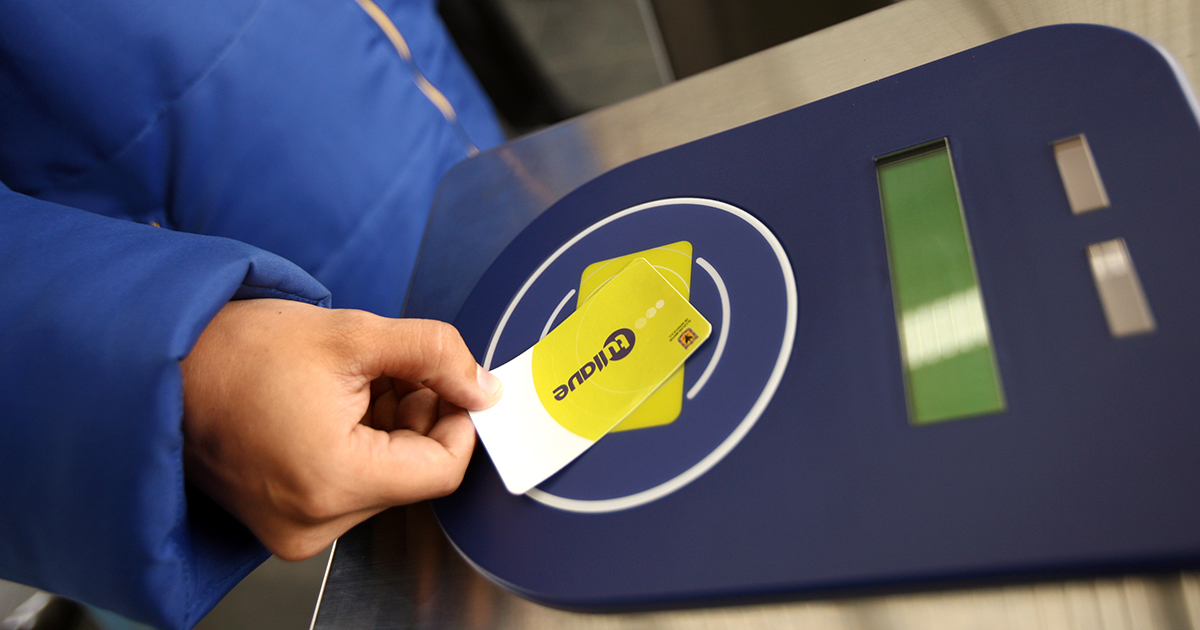
\includegraphics[width=80mm]{tfm-img8}}
\caption{La tecnología digital en los sistemas de reconocimiento.} \label{fig:señales}
\end{figure}

Nuevamente, la seguridad volvía a poner en duda los dispositivos empleados para contener la información de identificación de una persona. Los sistemas de reconocimiento basados en este tipo de dispositivos quedaban de esta manera expuestos a vulnerabilidades que podían desembocar en suplantaciones de indentidad. Todo esto era debido al gran avance tecnológico que se estaba produciendo, lo que hacía que sistemas que eran muy seguros en el momento de aparición de esa tecnología, con el paso del tiempo se conviertesen en obsoletos y débiles. Esto suponía que una nueva innovación en este sentido tendría una fuerte acogida al comienzo pero un nuevo declive con el paso del tiempo debido a los problemas de seguridad que se presentarían. \\

Este motivo hizo pensar en las características anatómicas que posee el ser humano como posible solución final a todos esos problemas. Esta propuesta cubría todas las condiciones que las anteriores no alcanzaban ya que presentaba propiedades de invariabilidad en el tiempo; lo que permitía que la persona mantuviera sus mismas características a lo largo de su vida, la imposibilidad de modificarlo o suplantarlo ya que son innatos a la persona que los tiene, etc. De todo esto surgió la idea de utilizar zonas del cuerpo humano como fuentes de información para los sistemas de reconocimiento a través de los patrones que estas describen. Así, partes de la fisiología de la persona como la huella dactilar, la retina, el iris, la palma de la mano e incluso la manera de andar constituían un gran almacen de datos que posibilitaría la identificación en los sistemas de reconocimiento. Con este nuevo medio de depósito de los datos, la seguridad, fiablidad y consistencia de la información aumentaba en los sistemas de información, quedando entonces del lado de ellos los errores que se produjeran por una mala identificación.  \\

El empleo de patrones de las características anatómicas del ser humano son la base de los actuales sistemas de reconocimiento. Estos se centran actualmente en mejorar los algoritmos empleados en el reconocimiento intentando conseguir una buena práctica y manejo de la información.   \\


\subsection{Reconocimiento de patrones}

El reconocimiento de patrones es la ciencia que se encarga de la descripción y clasificación (reconocimiento) de objetos, personas, señales, representaciones, etc. Esta ciencia trabaja en base un conjunto previamente establecido de todos los posibles objetos (patrones) individuales a reconocer. El ámbito de las aplicaciones basadas en el reconocimiento de patrones es muy amplio, siendo sin embargo las análogas al ser humano las que copan la mayor relevancia. El reconocimiento de patrones se da tanto en sistemas bióligicos como en sistemas dotados de inteligencia. Un claro ejemplo biológico lo vemos cuando en nuestro organismo los anticuerpos atacan a instrusos externos a los cuales reconoce a través del uso de patrones, en esta misma tesitura también se da el reconocimiento de patrones cuando nuestros oídos captan el habla y el sonido siendo capaz de interpretarlo. Del mismo modo, en situaciones que suceden en la naturaleza como cuando se produce la captura de las presas por parte de los animales se da el reconocimiento de patrones para conocer y diferenciar los tipos de presas. Este tipo de ejemplo llevado a los sistemas artificiales los podemos ver en los lectores de caracteres óptico (OCR) que son capaces de comprender el texto escrito y de como incluso las máquinas son capaces de enfrentarse a obstaculos y reconocer el diseño y características de estos. Cuando los patrones son de una naturaleza visual, el reconocimiento de patrones puede considerarse como un complemento en las técnicas de visión por computador proporcionando las capacidades de interpretación y clasificación \cite{Reference8}. \\

El reconocimiento de patrones esta ligado estrechamente con las redes neuronales. El nuevo interés a principios de los años 80 en las redes neuronales y el conexionismo como una alternativa al reconocimiento de patrones estadísticos y la inteligencia artificial (IA) puede atribuirse a dos factores. El primero es la realización que una función de aproximación de suficiente complejidad puede aproximarse a cualquier función objetivo con una precisión arbitraria. El segundo factor indica la capacidad para entrenar redes multicapas y no lineales usando backpropagation \cite{Reference8}. \\

Como se puede observar, el reconocimiento de patrones es la base teórica más importante de la biometría, de cómo esta busca la identidad de una persona en la forma de su mirada (la cara, la retina o el iris) o de algunas de sus zonas (las huellas dactilares o la geometría de la mano). En esencia, un sistema biométrico es un sistema de reconocimiento de patrones, razón por la cual el estudio de las bases matemáticas sobre las cuales se sustenta esta ciencia se vuelve de vital importancia para los fabricantes de tecnología biométrica. \\


\subsection{Componentes de los sistemas de reconocimiento de patrones}

El esquema de un sistema basado en el reconocimiento de patrones consta de varias etapas relacionadas entre sí (los resultados de una etapa pueden modificar los parámetros de etapas anteriores). La figura 2.4 muestra un esquema general de un sistema de reconocimiento de patrones en el cual el sensor tiene como propósito proporcionar una representación factible de los elementos del universo a ser clasificados en lo que se conoce como la etapa de adquisición de datos. Es conveniente realizar una etapa de preprocesamiento sobre cada uno de ellos en lugar de ser dados como entrada del sistema tal y como fueron obtenidos durante dicha etapa. La principal ventaja de realizar un preprocesamieno sobre los datos es que puede reducir la dimensionalidad de los mismos, lo cual mejora substancialmente la ejecución del sistema, sobre todo cuando se utiliza una metodología como la de redes neuronales. La extracción de características es la etapa que se encarga, a partir del patrón de representación de los datos, de extraer la información discriminatoria eliminando la información redundante e irrelevante. Es uno de los principales problemas que se dan en el reconocimiento de patrones, el encontrar una manera óptima de representar la información original que describe a cada uno de los patrones. Este proceso trata de reducir la cantidad de datos (reducción de dimensionalidad) que representa cada uno de los patrones, obteniendo de esta forma un vector de características que represente de la mejor manera posible al patrón original. El clasificador es la etapa de toma de decisiones en el sistema. Su rol es asignar los patrones de clase desconocida a la categoría apropiada. \\

En el caso de reconocimiento de patrones en imágenes la primera de las etapas, la adquisición de datos, generalmente es llevada a cabo mediante un dispositivo de captura de imagen, que se encarga de transformar la información obtenida del mundo real en un vector numérico que contiene los valores muestreados y cuantificados y que posteriormente es preprocesado. La etapa de selección y extracción de características es de suma importancia en un sistema de reconocimiento de patrones. Requiere un profundo análisis de los patrones para determinar que medidas son las cruciales en la identificación de las diferentes categorías. Durante esta etapa se aborda la recolección de información relevante proveniente de los dispositivos sensores para el proceso de clasificación. En el reconocimiento de patrones en imágenes se intenta extraer la información importante de las mismas en función del tipo de imagen, obviando siempre la que pueda ser intrascendente como el ruido. El objetivo final de un sistema de reconocimiento de patrones es la asignación automática de una categoría (o clase) a cada uno de los patrones de entrada \cite{Reference8}. \\

\begin{figure}[htbp]
\centering
\subfigure{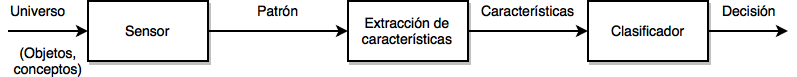
\includegraphics[width=140mm]{tfm-img9}}
\caption{Esquema general de un sistema de reconocimiento de patrones.} \label{fig:señales}
\end{figure}

El objetivo de estas etapas es ajustar el sistema para que sea capaz de clasificar señales u objetos de entrada en una de las clases predefinidas. Para ello deberá analizar un cierto número de características y para poder clasificar satisfactoriamente información de entrada es necesario un proceso de aprendizaje en el cual el sistema crea un modelo de cada una de las clases a partir de una secuencia de entrenamiento o conjunto de vectores de características de cada una de las clases. Generalmente se acepta que la secuencia de muestras de entrenamiento debe contener para cada una de las clases un mínimo de elementos igual a diez veces la dimensión de los vectores de características. El sistema de reconocimiento de patrones debe tener en cuenta las fuentes de variabilidad como son el ruido, rotaciones, cambio de escala y deformaciones, lo cual se logra incluyendo en la secuencia de entrenamiento patrones que hayan experimentado estas modificaciones. Este tipo de comportamiento se da en la etapa de clasificación, cuyo proceso de construcción suele denominarse como aprendizaje o entrenamiento, pudiendo ser este supervisado, en donde se realiza a partir de un conjunto de patrones del que no se conoce su clase; o no supervisado , los cuales requieren de la disposición de un conjunto de patrones denominado conjunto de entrenamiento, de los cuales se conoce su clase \cite{Reference8}.\\


\section{Biometría}

El concepto de biometría proviene de las palabras bio (vida) y metría (medida), refiriéndose por tanto a todo equipo biométrico que mide e identifica alguna característica propia de la persona. Se puede definir como una tecnología de seguridad basada en el reconocimiento de una característica física e intransferible de las personas, como por ejemplo la huella digital. Todos los seres humanos contienen características morfológicas únicas que los diferencian. La forma de la cara, la geometría de partes de nuestro cuerpo como las manos, nuestros ojos y tal vez la más conocida, la huella digital, son algunos rasgos que nos diferencian del resto de seres humanos.\\

La medición biométrica se ha venido estudiando desde hace mucho tiempo y es considerada en la actualidad como el método ideal y más fiable para la identificación humana. A través de la biometría se pueden medir y extraer las características anatómicas de una persona para obtener información y generar su patrón para poder emplearlo en su indentificación. \\


\subsection{Sistemas biométricos}

El gran avance que se ha producido en el desarrollo de las tecnologías de la información y la comunicación ha echo que sistemas tradicionales de reconocimiento como lectores de tarjetas, número secreto, etc. hayan adoptado esta evolución para dar paso a los sistemas biométricos. La autenticación mediante verificación biométrica está convirtiéndose en algo cada vez más habitual en los sistemas de seguridad, tanto privados como públicos, en la electrónica de consumo y en las aplicaciones de punto de venta (POS). Además de la seguridad, otro de los factores que está impulsando la verificación biométrica es la comodidad. \\

Un sistema biométrico se basa en las características que aporta la anatomía del ser humano, fundamentando sus desiciones de reconocimiento mediante los patrones que estas forman. Estos patrones son características morfológicas únicas y de comportamiento que todos los seres humanos tenemos y que nos diferencian de los demás. Propiedades como la forma de la cara, la geometría de partes de nuestro cuerpo como las manos nuestros ojos y la huella digital, son algunos rasgos que nos diferencian del resto de seres humanos.\\

Los sistemas biométricos pueden ser clasificados de diferentes maneras. Dependiendo del tipo de característica que se utilice para llevar a cabo de la identificación biométrica los podemos clasificar en dos grandes tipos; la biometría estática y la biometría dinámica. \\

La biometría estática engloba todas las características físicas que posee la persona como la huella dactilar, el iris del ojo, la palma de la mano, la cara, la oreja, etc. mientras que la biometría dinámica se basa en las características de comportamiento como la escritura, la firma, etc. 
Otra clasificación de los sistemas biométricos la podemos basar en el tipo de tecnología biométrica sobre la que se basan, donde podemos encontrar el reconocimiento de huella dactilar, reconocimiento de iris, reconocimiento de la geometría de la mano, reconocimiento de firma escrita y reconocimiento de voz.\\

Por la cuota de mercado que tienen estas tecnologías biométricas podemos clasificarlas según la información proporcionada por el International Biometric Group en el estudio realizado en enero de 2016 donde muestra la proporción del consumo de los diferentes tipos de sistemas biométricos.\\

\begin{figure}[htbp]
\centering
\subfigure{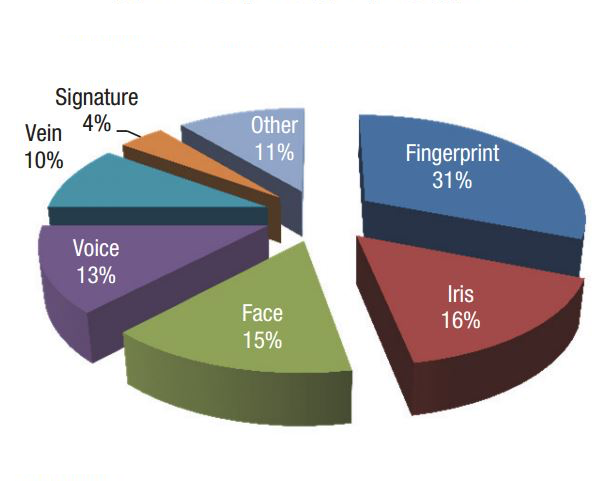
\includegraphics[width=80mm]{tfm-img10}}
\caption{Cuota de mercado de las modalidades de sistemas biométricos.} \label{fig:señales}
\end{figure}

En la figura anterior podemos ver como el reconocimiento por huella dactilar es el sistema biométrico más utilizado en el mercado por las aplicaciones de seguridad, teniendo el resto de tecnologías biométricas un alcance similar en cuanto al consumo. Esto no hace más que representar el desafío que supone el analizar e investigar un sistema biométrico que no esta tan asentado en el mercado como es el basado en el iris, y que puede conllevar a obtener nuevos hallazgos y soluciones que mejoren las capacidades de lo ya existente.


\subsection{Anatomía del iris}

El ojo es el órgano de la visión. Los ojos pueden distinguir variaciones muy pequeñas de forma, color, luminosidad y distancia. En realidad, el órgano que efectúa el proceso de la visión es el cerebro; la función del ojo es traducir las vibraciones electromagnéticas de la luz en un determinado tipo de impulsos nerviosos que se transmiten al cerebro. \\

El ojo en su conjunto, llamado globo ocular, tiene un diámetro aproximado de 2,5cm con un marcado abombamiento sobre su superficie delantera. Entre la pared del globo ocular y el hueso orbitario existe un tejido conjuntivo que une ambas estructuras. A dicha zona de unión se le conoce como cápsula de Tenon. \\

El ojo se compone de una serie de estructuras entre la que destacamos el iris, una membrana coloreada y de forma circular. Su coloración representa lo que conocemos habitualmente como “color de los ojos” y su apertura central es la pupila. Esta membrana presenta un músculo de disposición circular que permite modificar el tamaño de la pupila.\\

El iris forma parte de la capa media o úvea. Es un disco pigmentado que se encuentra a continuación del cuerpo ciliar, suspendido entre la córnea y el cristalino. Posee un orificio central conocido como pupila por donde pasan los rayos lumínicos tras haber atravesado la córnea y el humor acuoso. A través de la pupila los rayos llegan a la lente del cristalino, seguidamente al cuerpo vítreo y finalmente a las células receptoras de la retina para la formación de la imagen. El tamaño de la pupila depende de dos músculos que rodean sus bordes y controlan la cantidad de luz que entra en el ojo. Las fibras musculares del iris se agrupan formando dos músculos obiculares: el Esfínter del iris que produce la Miosis, y el dilatador de la pupila que produce la Midriasis. Si los músculos orbiculares del iris se contraen, la pupila se encoge y entra menos luz en el ojo (Miosis). Si los músculos orbiculares se relajan, la pupila vuelve a dilatarse, dejando pasar más luz a la retina (Midriasis).  La contracción pupilar se debe  a la acción de los esfínteres del iris y su objetivo es dar una imagen nítida, evitando para ello el paso de rayos por la periferia de la lente. El componente principal del iris es un tejido conjuntivo rico en células pigmentadas llamadas melanóforos.\\

Se encuentra situado entre la cámara anterior y posterior de un líquido gelatinoso llamado humor acuoso. La cámara anterior esta delimitada por la cara posterior de la córnea y la cara anterior del iris, mientras que la cámara posterior lo está por la cara posterior del iris y la cara anterior del cristalino. Posterior al cristalino se encuentra el humor vítreo que da volumen al globo ocular. \\

\begin{figure}[htbp]
\centering
\subfigure{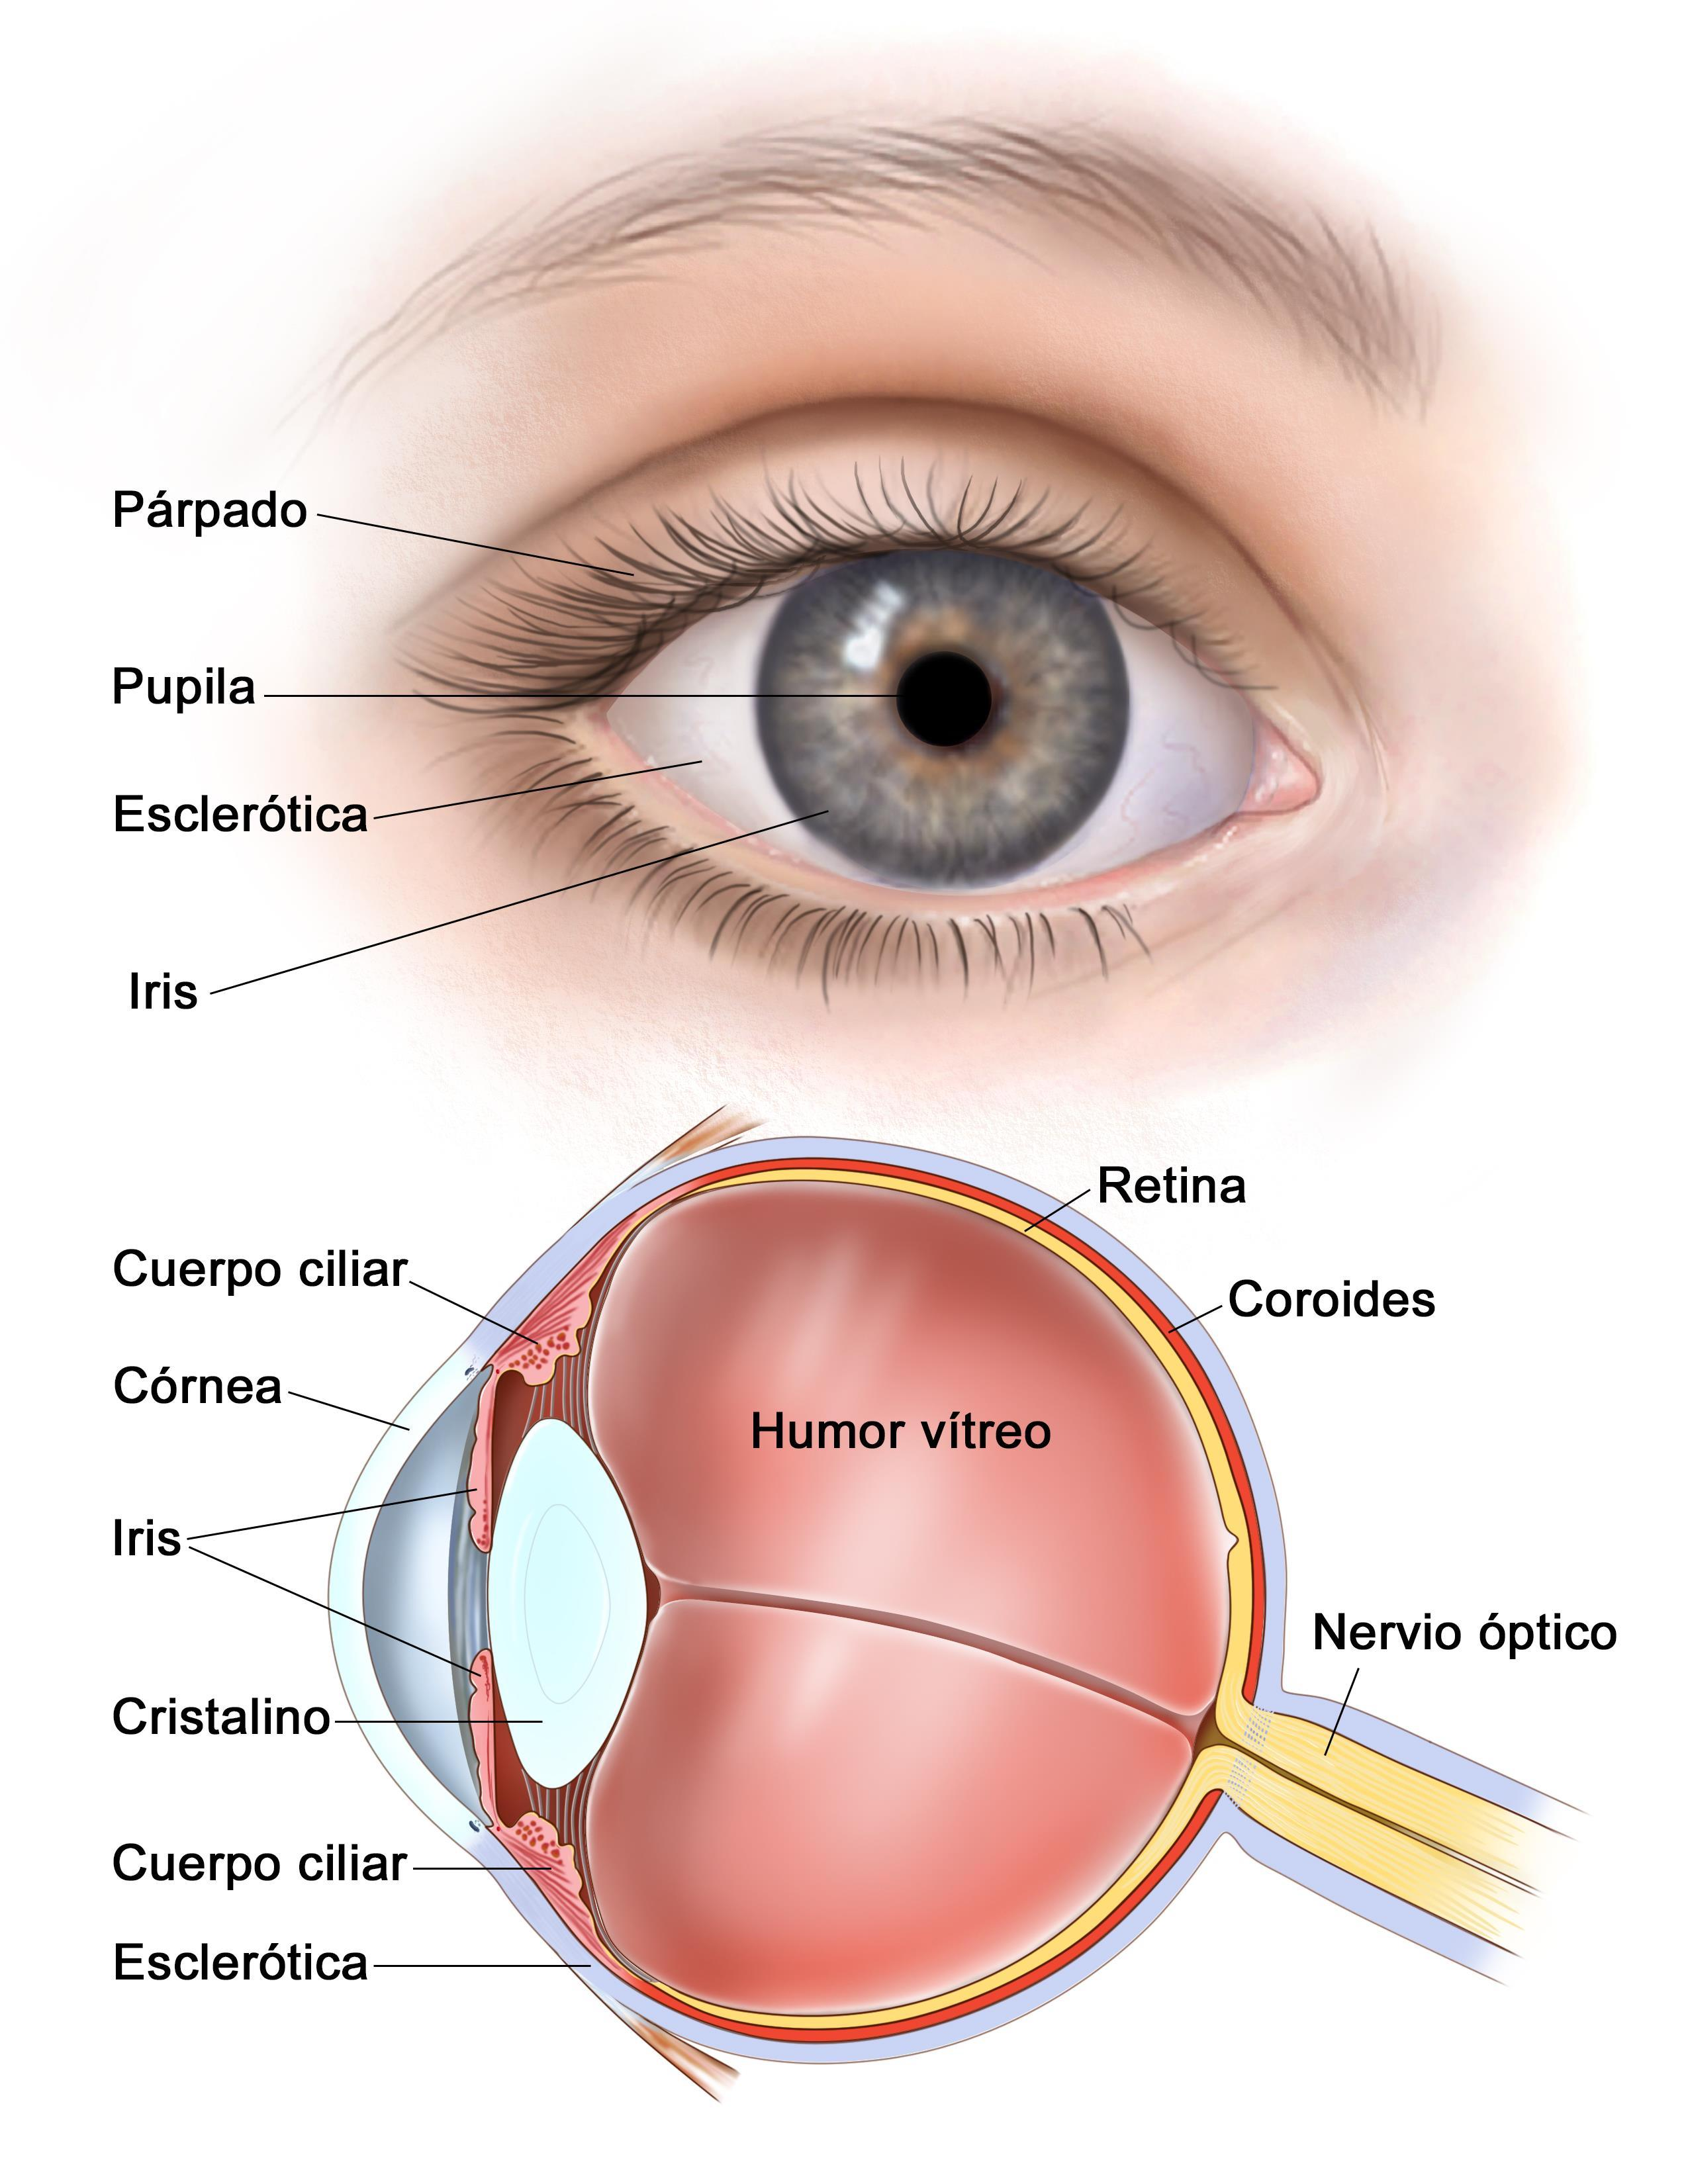
\includegraphics[width=80mm]{tfm-img11}}
\caption{Anatomía del iris.} \label{fig:señales}
\end{figure}

El iris es una zona delicada del ojo y que está expuesta a sufrir posibles daños y enfermedades. Los traumatismos son la causa mas frecuente de cataratas unilaterales en individuos jóvenes. Una herida contusa por la cual una contusión puede dar lugar a una “impronta” del pigmento del iris sobre la cápsula anterior del cristalino, así como opacidades corticales con forma de flor. La mayor temperatura del iris respecto a la de la córnea puede formar corrientes en termoconvección en el humor acuoso que ascienden y descienden cerca del iris y endotelio respectivamente. Son típicos en la mitad inferior de la córnea formando un triángulo con base inferior. El crecimiento o protuberancia en la superficie anterior del iris, que no son sino cúmulos inflamatorios en el parénquima iridiano, puede dar lugar a la enfermedad denominada Nódulos de Bussaca. \\

El color del iris está determinado por el número y distribución de unas células que contienen el pigmento Melanina y se llaman Melanocitos. Si la melanina se encuentra solamente en la zona de epitelio pigmentario de la superficie posterior del iris, el ojo es azulado. En cambio si esta se distribuye por todo el espesor del iris, el ojo es de color marrón. \\


%----------------------------------------------------------------------------------------


\section{Reconocimiento de iris}

A pesar de no ser el tipo de reconocimiento que mayor uso tiene en el mercado, este tipo de reconocimiento presenta una gran popularidad debido a las propiedades que posee como son principalmente los muchos grados de libertad con los que es dotada su textura, y el permanecer invariable en el tiempo a pesar del envejecimiento natural de la persona. Todo esto convierte al iris en una de las mas importantes características de la fisiología humana que da lugar a un sistema de reconocimiento biométrico robusto, fiable u seguro. \\

El proceso de reconocimiento de iris se compone de cuatro etapas principales: la adquisición de imagen, el pre-procesamiento, la  extracción de características y la comparación de las mismas. Estas cuatro fases constituyen una arquitectura de flujo de trabajo pipeline, donde el resultado de la salida de un etapa es la entrada en la inmediatamente posterior.\\

\begin{figure}[htbp]
\centering
\subfigure{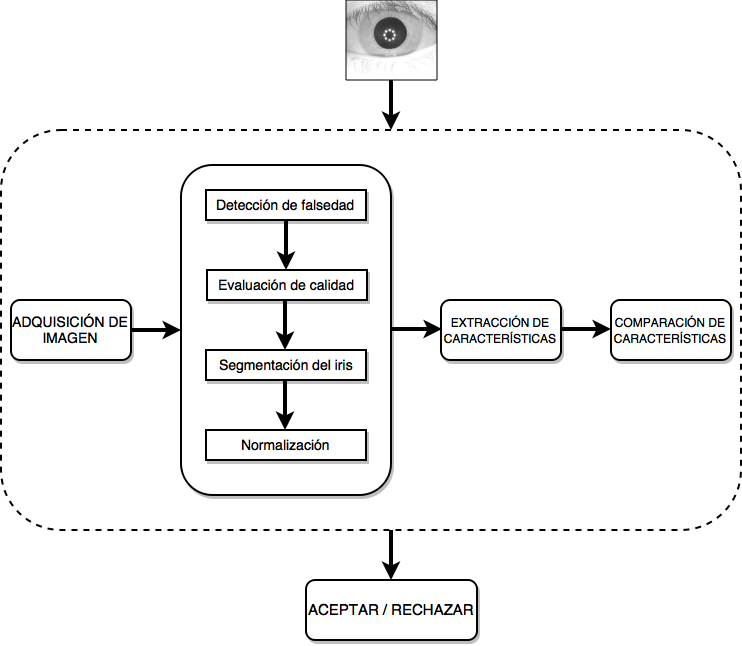
\includegraphics[width=130mm]{tfm-img12}}
\caption{Diagrama de flujo de un sistema de reconocimiento de iris.} \label{fig:señales}
\end{figure}


\subsection{Etapas del reconocimiento de iris}

Un sistema de reconocimiento basado en el iris se compone de cuatro etapas: adquisición de imagen, pre-procesamiento, extracción de características y comparación de características. En la figura 2.7 podemos ver el digrama del flujo de ejecución de un sistema de reconocimiento de iris convencional, los cuales comienzan con la adquisición de la imagen del iris y terminan aceptando o rechazando la identidad reclamada. \\

La primera etapa de adquisición de imagen es la encargada de capturar una secuencia de imágenes de iris. Estas capturas se realizan con cámaras especiales que suelen operar en el espectro visible (380-750 mm) o en el espectro infrarrojo (700-900 mm). En este ámbito, los sistemas de adquisición en el espectro infrarrojo son los más utilizados debido a las ventajas que proporciona. Dicho proceso de adquisición consiste en 2 operaciones: muestreo y cuantización. El muestreo está relacionado con la creación de la imagen digital, que tiene una resolución espacial predefinida con un número de pixeles por pulgada en función de la escena donde se realice. A través de la operación de cuantización, la señal de entrada es discretizada para obtener los posibles valores de intensidades de los pixeles que conforman la imagen. \\

La etapa de pre-procesamiento es la segunda y como se ha podido ver en la figura 2.7 se compone a su vez de 4 sub-etapas: detección de falsedad, evaluación de calidad de la imagen, segmentación del iris y normalizaciónd de la región del iris. La detección de falsedad es empleada para diferenciar entre un reclamo de identidad real y un falso reclamo con una imagen impresa de un iris, una grabación de secuencia de vídeo de un iris, ojos artificiales, lentes de contacto impresos con patrones de iris por ejemplo. Para detectar esa falsedad de identidad se emplean técnicas de medición de indicadores de espécimen vivo. La sub-etapa de evaluación de calidad dentro de la etapa del pre-procesamiento involucra varios factores de calidad como son: emborronado por desenfoque, emborronado por movimiento, dilatación de la pupila, área útil del iris, reflexiones especulares, variaciones de iluminación, oclusión por pestañas y párpados. Una pronta detección y corrección de estos factores de calidad ayudará a que el proceso de reconocimiento del iris sea mas robusto, aunque existen muchos sistemas de reconocimento de iris que imponen una serie de restricciones en la etapa de adquisición de la imagen del iris teniendo como objetivo el reducir dichos factores de calidad. \\

La segmentación del iris se compone también de una serie de pasos: encontrar un iris en la imagen, demarcar sus bordes interno y externo entre la pupila y la esclerótica respectivamente, detección de los bordes de los párpados superior e inferior si estos ocluyen el iris, y detectar y excluir cualquier objeto superpuesto de pestañas o reflexiones de la córnea o gafas. Existen diferentes métodos propuestos de segmentación de iris como: método basado en el operador integro-diferencial, método basado en la transformada de Hough, método basado en el análisis de contornos activos, método basado en la teoría de juegos, etc. Con el paso de la normalización de lo que se trata es de solucionar los problemas relacionados con las dimensiones de la imagen del iris. La dimensión de la imagen del iris puede variar de un individuo a otro o en el mismo individuo debido a la variación de la pupila, la variación de la distancia entre el individuo y la cámara, el movimiento del ojo, la inclinación de la cabeza, etc. Con el proceso de normalización lo que se hace es transformar la región segmentada del iris en un sistema de coordenadas pseudo-polar de 2 dimensiones mediante un muestreo de los datos originales en un tamaño predefinido. Aunque en algunos modelos del desarrollo de extracción de características no se realiza este proceso para ahorrar en coste computacional, el modelo "rubber sheet" es el método mas usado para la normalización \cite{Reference9}. \\

En la siguiente etapa se extraen las características mas significativas y relevantes de la textura de la imagen del iris. Este proceso se ha desarrollado utilizando diversos algoritmos de codificación entre los que se pueden destacar: banco de filtros espaciales, transformada de Gabor wavelets en 2 dimensiones, transformada discreta de los cosenos, transformada discreta de Fourier en 2 dimensiones, características ordinales, descriptores SIFT alrededor de un punto de interés, etc. El éxito de las estapas de segmentación y extracción de características se encuentra estrechamente ligado a los factores de calidad de la imagen del iris, por lo que como se ha mencionado anteriormente, una buena etapa de pre-procesamiento puede evitar que se dé el caso en el que usuarios auténticos  con imágenes capturadas con mala calidad puedan ser injustamente rechazados ya que difieren de sus plantillas biométricas registradas. \\

Por último, en la etapa de comparación de característica se confirma si la imagen de la textura del iris de un individuo dado se corresponde a algunas de las identidades registradas por el sistema. Esta operación de similitud se desarrolla utilizando diferentes medidas de similitud propuestas en función de la magnitud de las características extraidas. Mediante estas medidas de magnitud se puede decidir si la identidad reclamada es aceptada o rechazada. Entre las medidias más utilizadas en la comparación de características de la textura del iris se pueden destacar: distancia euclidiana, distancia de Hamming o la función BLPOC \cite{Reference9}.\\


\section{Reconocimiento de iris en condiciones no ideales}

La mayor parte de los trabajos realizados sobre el reconocimiento del iris alcanzan muy buenos resultados que se convierten en casi inalcanzables en ambientes deseados. Como se ha mencionado anteriormente, en la actualidad son muchas las investigaciones que se centran en el desarrollo de métodos robustos capaces de realizar un reconocimiento del iris en ambientes no deseados o condiciones no ideales. La tendencia de esta modalidad de reconocimiento biométrico viene promovida por la necesidad de algunas aplicaciones reales para obtener una mayor flexibilidad frente a situaciones como: seguimiento de personas, reconocimiento de personas en multitudes, control de acceso, etc, donde la aparición de factores de calidad como iluminación, escala, oclusión y/o perspectiva convierten el entorno del reconocimiento en no deseado, teniéndose este que realizar en condiciones no ideales. A pesar del gran avance de los desarrollos producido en este campo, existen actualmente grandes retos en cuanto al reconocimiento de iris en condiciones no ideales \cite{Reference9}.\\

El reconocimiento del iris en condiciones no ideales se caracteriza por manifestarse en situaciones donde el individuo se encuentra en constante movimiento o en escenarios con presencia de objetos y/u otros individuos, lo que provoca que se realicen capturas de imágenes del iris afectadas por factores de calidad. Se suelen dar una serie de factores de calidad comunes a las imagenes capturadas este tipo de situaciones como son la iluminación variable, el emborronado, la oclusión, la reflexión especular, el tamaño del área del iris y la perspectiva. \\
 
La existencia de estos factores de calidad en las imagenes del iris pueden producir que la medida de éxito de los sistemas de reconocimiento se vea afectada negativamente. Por este motivo suelen aperecer una serie decisiones que se pueden tomar para intentar mitigar este problema como son el descartar las imagenes que no superen un umbral de índice de calidad establecido, el aplicar técnicas para mejorar la calidad de las imágenes, el desarrollar técnicas mas robustas de reconocimiento de iris en imagenes de mala calidad y el obtener combinaciones de estas técnicas \cite{Reference9}.\\

\begin{figure}[htbp]
\centering
\subfigure{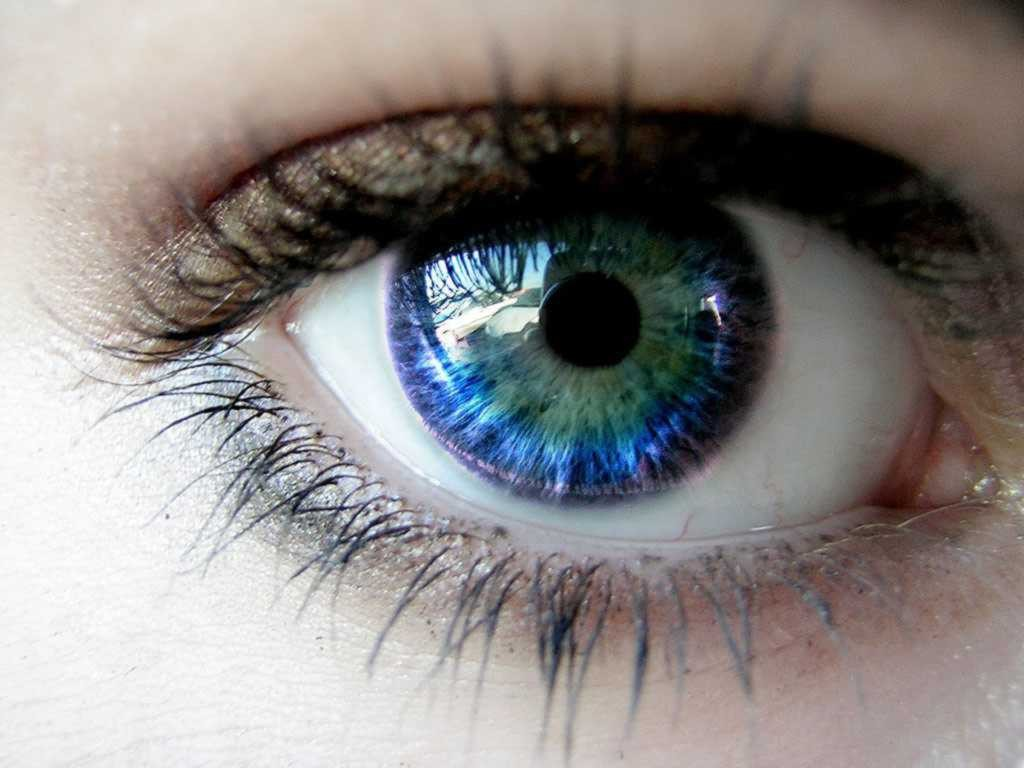
\includegraphics[width=44mm]{tfm-img13}}
\subfigure{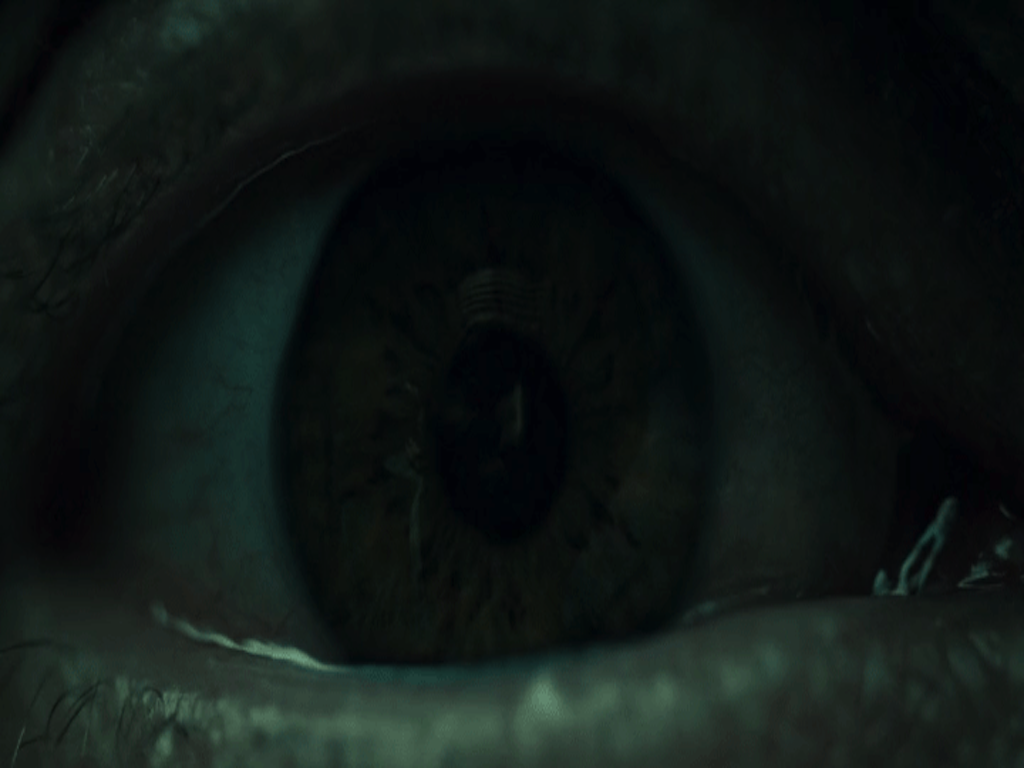
\includegraphics[width=44mm]{tfm-img14}}
\subfigure{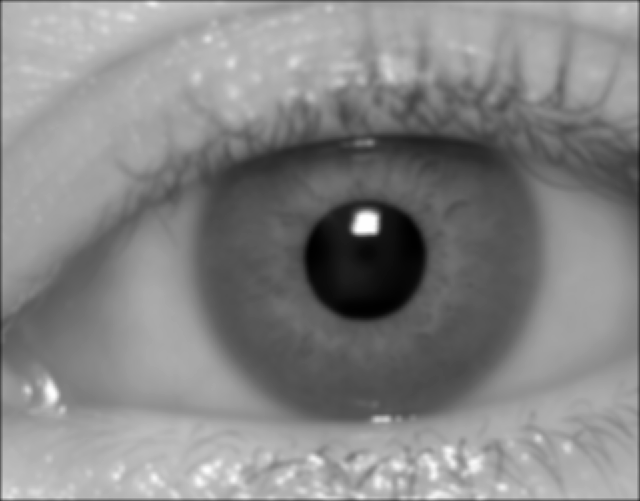
\includegraphics[width=60mm]{tfm-img15}}
\caption{Imágenes de iris afectadas por factores de calidad.} \label{fig:señales}
\end{figure}


\subsection{Factores de calidad}

En esta sección describiremos los factores de calidad más comunes que suelen aparecer en las imágenes de textura del iris cuando estas se realizan en movimiento o con la presencia de objetos y/o personas. \\

La iluminación variable es un problema que está estrechamente ligado a la localización de la fuente de luz con respecto al dispositivo de captura y el individuo que se quiere reconocer. Estas variaciones de iluminación están siempre relacionadas al movimiento de la persona con respecto a las fuentes de luz. Debido a esto, la intensidad y la dirección de las fuentes de iluminación pueden afectar la apariencia de imágenes del iris e indicir en las medidas de éxito de los sistemas de reconocimiento de iris. Algunos sistemas de reconocimiento emplean el uso de filtros ópticos para reducir el efecto de la luz variable, ya que estos bloquean con luz estroboscópica una gran porción de luz ambiental. La aplicación de técnicas de ecualización de histogramas y  de estandarización es otro método utilizado para disminuir el efecto contraproducente de la variabilidad luminosa. \\

Como hemos visto en la sección \textbf{Anatomía del iris}, este se representa como un anillo que tiene el borde inferior situado sobre la pupila y el borde exterior sobre la esclerótica, siendo su función principal la de controlar el tamaño de la pupila en función de la cantidad de luz que entra en el ojo a través de esta.  Esa cantidad de luz puede dar lugar a que se den dos fénomenos en la pupila; la "Miosis" debido a que la pupila se contrae por el exceso de cantidad de luz y la "Midriasis" que se dilata por el efecto contrario, es decir, poca cantidad de luz. La variabilidad de tamaño de la pupila hace el tamaño de la región del iris pueda variar. \\

En situaciones en las que se capture la imagen del iris con mucha cantidad de luz provocará que la pupila esté dilatada, dando lugar a que no se obtenga la información necesaria para realizar el proceso de reconocimiento. Esto es debido a que la dilatación de la pupila produce una deformación y pérdida de información relevante del patrón estructural del iris \cite{Reference9}.\\

El problema que produce el efecto de emborronado sobre las imágenes es causado principalmente por 2 motivos como son los movimientos significativos del individuo respecto al dispositivo de captura o del dispositivo de captura respecto al individuo en el momento de la adquisición de la imagen y que el punto focal del objeto a capturar esté fuera de la profundidad del campo del dispositivo de captura de la imagen. Para paliar este problema se han desarrollado soluciones basadas en enfoques de estabilización opto mecánica que va incorporada en el ensamblado de las lentes de las cámaras utilizando un software conectado con un control electrónico de imagen. Estas soluciones implican la incorporación de dispositivos costosos y voluminosos que no serían viables para ser utilizados en aplicaciones móviles. En este sentido, se han propuesto varios métodos que permiten entre otras cosas  determinar el nivel de afectación de emborronado  en las imágenes, así como medir el foco de una imagen por el análisis de la nitidez del límite entre el iris y la pupila. \\

Otro de los factores de calidad que se puede dar en las imágenes de captura de iris es el referente a la oclusión ocasionada por los párpados y pestañas, las cuales pueden ser parciales o totales. En este caso, en las oclusiones parciales se puede comprobar como la oclusión al iris se produce mayormente por el párpado y las pestañas superiores. Esta situación es muy común en los seres humanos, ya que con el paso de los años el párpado tiende a caerse y con ello a obstruir el ojo. Por otro lado, las oclusiones totales se deben en parte a algún tipo de enfermedad padecida por el individuo o alguna fuerte reacción a cambios en el ambiente. El efecto de oclusión provoca que se capturen imágenes que proporcionen poca o ninguna información de los patrones estructurales del iris, afectando con ello a la medida de éxito de los sistemas de reconocimiento de iris \cite{Reference9}.\\

Al igual que con los anteriores factores de calidad, son varias las soluciones desarrolladas para la detección de párpados y pestañas entre los que se encuentran el método de detección de párpados y pestañas basado en las transformada de Hough \cite{Reference10} o el método de detección de párpados basado en características de las frecuencias de las pestañas \cite{Reference11} entre otros. \\

La reflexión especular es un factor de calidad que viene asociado a los mecanismos de iluminación que traen incorporados los dispositivos de captura de imagen del iris para iluminar el ambiente en el que se encuentra el individuo que vaya a ser reconocido para poder capturar imágenes de iris con mayor calidad y grado de detalle posible. Este medio propicia que se produzcan reflexiones de luz sobre la córnea del ojo del individuo. Estas reflexiones especulares pueden ser definidas como manchas blancas que ocluyen y esconden información del iris y la pupila. Esta oclusión de información por parte las reflexiones especulares sobre el iris puede provocar que se altere el patrón estructural de este, llegando en ocasiones a no poder localizarlo. Esto puede ocasionar que un individuo sea rechazado por el sistema de reconocimiento aún estando registrado por dicho sistema \cite{Reference9}. \\

Existen varias soluciones para evitar que aparezcan reflexiones especulares en las imágenes del iris, siendo una de ellas la de controlar la iluminación ambiental con iluminación NIR. Aunque otros trabajos desarrollados proponen otro tipo de soluciones basados en un sistema con una fuente de luz menos invasiva diseñado para eliminar reflexiones especulares \cite{Reference12}. \\

El factor de la perspectica se encuentra relacionado con la desviación de la mirada del individuo a reconocer respecto a la vista frontal ideal desde el dispositivo de captura. Este factor tiene una enorme influencia sobre la medida de éxito de los sistemas de reconocimiento de iris, ya que las imágenes de iris con desviaciones respecto a la vista frontal ideal tienen la característica de que el iris capturado posee una forma elíptica. Esto hace que el patrón estructural del iris tienda a deformarse significativamente, lo que produce que la información capturada del mismo no coincida con el modelo estructural de un iris normal \cite{Reference9}. \\  

Existen varios trabajos desarrollados para procesar este tipo de imágenes como el propuesto por J. Zhu y J. Yang \cite{Reference13} basado en la estimación de la dirección de la mirada sobre el análisis de secuencias de vídeo, y también Dorairaj et al. en \cite{Reference14} estiman el ángulo de desviación de la mirada repecto a la vista frontal ideal optimizando una función objetivo basada en la distancia de Hamming \cite{Reference15}. \\

%----------------------------------------------------------------------------------------